\documentclass[11pt,a4paper]{article}

% ---- Packages ---------------------------------------------------------------
\usepackage[T1]{fontenc}
\usepackage[utf8]{inputenc}
\usepackage{lmodern}
\usepackage{microtype}
\usepackage{amsmath,amssymb,amsthm}
\usepackage{bm}
\usepackage{booktabs}
\usepackage{graphicx}
\usepackage{hyperref}
\usepackage{cleveref}
\usepackage{algorithm}
\usepackage{algpseudocode}
\usepackage{listings}
\usepackage{xcolor}
\usepackage[margin=2.5cm]{geometry}
\usepackage{natbib}
\usepackage{caption}
\usepackage{subcaption}
\usepackage{tikz}
\usetikzlibrary{arrows.meta,positioning,shapes.geometric}

% ---- Theorem environments ---------------------------------------------------
\newtheorem{theorem}{Theorem}
\newtheorem{proposition}[theorem]{Proposition}
\newtheorem{lemma}[theorem]{Lemma}
\newtheorem{definition}{Definition}
\newtheorem{remark}{Remark}

% ---- Maths macros -----------------------------------------------------------
\newcommand{\R}{\mathbb{R}}
\newcommand{\E}{\mathbb{E}}
\newcommand{\KL}{\mathrm{KL}}
\newcommand{\N}{\mathcal{N}}
\newcommand{\Lap}{\mathcal{L}}
\newcommand{\I}{\mathcal{I}}
\newcommand{\A}{\mathcal{A}}
\newcommand{\diag}{\mathrm{diag}}
\newcommand{\tr}{\mathrm{tr}}
\newcommand{\lse}{\mathrm{lse}}
\newcommand{\elbo}{\mathcal{L}}
\newcommand{\bLambda}{\bm{\Lambda}}
\newcommand{\bU}{\bm{U}}
\newcommand{\bS}{\bm{S}}
\newcommand{\bW}{\bm{W}}
\newcommand{\bz}{\bm{z}}
\newcommand{\bmu}{\bm{\mu}}
\newcommand{\bomega}{\bm{\omega}}
\newcommand{\bx}{\bm{x}}
\newcommand{\bX}{\bm{X}}
\newcommand{\bE}{\bm{E}}
\newcommand{\bL}{\bm{L}}
\newcommand{\bK}{\bm{K}}

% ---- Shorthand for the model name ------------------------------------------
\newcommand{\VDT}{VDT\xspace}
\newcommand{\vdt}{Vibrational Wiring Deduction Transformer\xspace}
\newcommand{\WA}{WiringAutoencoder\xspace}  % predecessor shorthand

% ---- Code style -------------------------------------------------------------
\lstset{
  basicstyle=\ttfamily\footnotesize,
  keywordstyle=\color{blue!80!black},
  commentstyle=\color{gray},
  stringstyle=\color{teal},
  backgroundcolor=\color{gray!8},
  frame=single,
  breaklines=true,
  language=Python,
  numbers=left, numberstyle=\tiny\color{gray},
  xleftmargin=1.5em,
}

% ---- Title ------------------------------------------------------------------
\title{%
  \textbf{Vibrational Wiring Deduction Transformer (VDT):}\\[4pt]
  \large A Spectral-PPCA Generative Framework for\\[2pt]
  Graph-Structured Latent Spaces and Spectral Associative Memory
}

\author{%
    Lorenzo Moriondo\\
    \small Independent Researcher --- tuned.org.uk\\
    \small ORCID: 0000-0002-8804-2963\\
    \href{https://github.com/tuned-org-uk/vibrational-deduction-transfomer}{\texttt{github repo}}
}

\date{June 2026}

% =============================================================================
\begin{document}
\maketitle

\begin{abstract}
We present the \emph{Vibrational Wiring Deduction Transformer} (VDT), a
fully Bayesian generative model that unifies vibrational graph dynamics,
probabilistic PCA in a Laplacian eigenbasis (Spectral-PPCA), and spectral
associative memory into a single trainable architecture.  The predecessor
\WA{} used a hard high-frequency energy penalty
($J_{\mathrm{freq}}$) and an isotropic Gaussian latent prior.  VDT replaces
both with principled variational KL terms: (i) a spectral-basis KL over the
loading matrix $\bS$ weighted by Laplacian eigenvalues, implementing a
\emph{spectral Occam's razor}; (ii) a closed-form Gamma/Exponential KL over
per-mode weights $\bomega$, providing soft $\tau$-mode band-limiting; and
(iii) the standard isotropic Gaussian latent KL retained for stability (the
Laplacian-precision latent KL is preserved as a design option and ablation,
but is not included in the default three-term ELBO following architectural
review in PR\,\#35).  After training, a \emph{spectral artefact} $\A(\I)$ is
extracted and used to initialise a downstream transformer with pre-built
spectral associative memory.  The two-phase (offline training, online
inference) architecture separates spectral learning from deployment, with
frozen eigenpairs eliminating all runtime $O(N^3)$ eigendecompositions during
training.  We detail the complete module design, three-term ELBO, stability
analysis, benchmark metrics, and associative memory construction.
\end{abstract}

% ---- ToC --------------------------------------------------------------------
\tableofcontents
\newpage

% =============================================================================
\section{Introduction}
\label{sec:intro}

Graph-structured latent variable models occupy an increasingly important niche
between classical variational autoencoders (VAEs) and geometric deep learning:
they can encode both the \emph{content} of nodes and the \emph{relational
structure} that organises them.  The \WA{}~\citep{vdt_v1}
recognised this, using a differentiable graph Laplacian $L(z)$ as an
intermediate latent object whose spectral properties are regularised by a hard
frequency penalty $J_{\mathrm{freq}} = \sum_{j>k}\lambda_j(L(z))$.  While
effective in practice, this penalty is a heuristic rather than a proper
probabilistic prior, which makes it difficult to:
\begin{enumerate}
  \item compare competing ArrowSpace indices $\I_1, \I_2$ via principled model
        selection;
  \item interpret the learned spectral structure as a posterior over loading
        matrices $\bW$;
  \item extract a reusable \emph{spectral artefact} whose keys are
        approximately orthonormal and whose values are grounded in the data
        manifold.
\end{enumerate}

The VDT addresses all three limitations by embedding the \WA{}
within the Spectral-PPCA framework~\citep{design_a}, a Bayesian
generative model in which the loading matrix
$\bW = \bU_{1:q}\,\diag(\bomega)\,\bS$ lives explicitly in the Laplacian
eigenbasis and is endowed with eigenvalue-weighted shrinkage priors.  The VDT
encoder backbone implements a discrete damped wave equation in the graph
spectral domain, connecting the probabilistic latent space to the physical
intuition of vibrational modes in string and spring systems.

\subsection{Contributions}
\begin{itemize}
  \item A three-term ELBO replacing $J_{\mathrm{freq}}$ and preserving the
        isotropic latent prior (Section~\ref{sec:elbo}).
  \item A \texttt{SpectralLoadingDecoder} that maps latent codes to
        eigenbasis-factorised loading matrices
        (Section~\ref{sec:modules}).
  \item A \texttt{VibrationalEncoder} (VDT recurrence) with
        \texttt{ModeWeightHead} producing variational Gamma parameters
        (Section~\ref{sec:modules}).
  \item A \texttt{SpectralAssociativeMemory} module that pre-builds a
        Hopfield memory from the spectral artefact
        (Section~\ref{sec:memory}).
  \item A two-phase offline/online architecture eliminating runtime
        eigensolves during training (Section~\ref{sec:two_phase}).
  \item An eight-metric evaluation suite including ELBO Bayes factors for
        ArrowSpace index selection (Section~\ref{sec:benchmarks}).
\end{itemize}

% =============================================================================
\section{Background}
\label{sec:background}

\subsection{Probabilistic PCA}

Standard PPCA~\citep{tipping1999ppca} defines a linear-Gaussian generative
model:
\begin{equation}
  \bz \sim \N(\mathbf{0}, \bm{I}_q), \qquad
  \bx \mid \bz \sim \N(\bW\bz + \bmu,\, \sigma^2 \bm{I}_d),
  \label{eq:ppca}
\end{equation}
producing marginal $\bx\sim\N(\bmu,\,\bW\bW^\top+\sigma^2\bm{I}_d)$.
Maximum-likelihood estimation recovers the PCA loading matrix in the column
space of the $q$ largest singular vectors of the data matrix.  The fully
Bayesian extension places priors over $\bW$, $\bz$, and $\sigma^2$, enabling
model selection over the latent dimensionality $q$ via the marginal
likelihood~\citep{minka2001pca}.

\subsection{Graph Laplacian Spectral Theory}

Let $G=(V,E,w)$ be a weighted graph with node set $|V|=N$.  The normalised
graph Laplacian is $L = D^{-1/2}(D-W)D^{-1/2}$ where $D_{ii}=\sum_j w_{ij}$.
Eigendecomposition $L = \bU\bLambda\bU^\top$ yields eigenvectors
$\bU=(\mathbf{u}_1,\dots,\mathbf{u}_N)\in\R^{N\times N}$ and non-negative
eigenvalues $0\le\lambda_1\le\cdots\le\lambda_N$.  Low-frequency eigenvectors
(small $\lambda_k$) are smooth over $G$; high-frequency ones (large $\lambda_k$)
oscillate rapidly across edges~\citep{chung1997spectral}.

Given ArrowSpace index $\I$, we denote the frozen $q$-truncated eigendecomposition
\begin{equation}
  L(\I) = \bU\bLambda\bU^\top,
  \qquad
  \bU_q = \bU_{:,1:q}\in\R^{N\times q},
  \qquad
  \bLambda_q = \diag(\lambda_1,\dots,\lambda_q).
  \label{eq:eig}
\end{equation}
These eigenpairs are computed once offline and used as frozen constants
throughout training.

\subsection{Vibrational Dynamics and Spectral Graph Waves}
\label{sec:vibration}

The VDT encoder draws its physical motivation from Rayleigh's Theory of
Sound~\citep{rayleigh1877sound}: the eigenmodes of a vibrating string or spring
system are exactly the eigenvectors of the system's stiffness matrix, which in
the discrete graph setting is the normalised Laplacian $L$.  A positive
amplitude on mode $k$ corresponds to a string displacement in the direction
$\mathbf{u}_k$; a negative amplitude corresponds to the opposing displacement.
This is the physical counterpart to the signed (positive/negative) latent
amplitudes that the VDT encoder learns.

The signed density matrix
$\varrho_t = \varrho_t^+ - \varrho_t^-$ maintained by the VDT recurrence
(Section~\ref{sec:encoder}) is precisely a decomposition of the current state
into constructive and destructive vibrational contributions.  The low-entropy
state of this system corresponds to coherent oscillation (the string vibrating
in a definite mode); the high-entropy state corresponds to rest (the wave
function collapsed, all modes equally weighted).  This mirrors Brownian
motion, where the low-entropy state is the non-heated stationary system and
the high-entropy state is maximal thermal agitation.

\subsection{WiringAutoencoder (Predecessor)}
\label{sec:wa_v1}

The \WA{}~\citep{vdt_v1} trains a differentiable Laplacian $L(\bz)$ whose
topology is fixed (kNN + RBF graph) but whose edge weights are learned by a
mixture-of-experts decoder $W_{\mathrm{dec}}:\bz\mapsto\delta_e$.  The
training objective is
\begin{equation}
  \elbo_{\mathrm{WA}} =
    \E_q[\log p(\bx\mid\bz)] -
    \beta\cdot\KL(q(\bz)\|\N(\mathbf{0},\bm{I})) -
    \alpha\cdot J_{\mathrm{freq}}(L(\bz)),
  \label{eq:wa_elbo}
\end{equation}
where $J_{\mathrm{freq}} = \sum_{j>k}\lambda_j(L(\bz))$ penalises
high-frequency wiring.  The reconstruction is provided by
\texttt{TauModeDiffusion}: the heat kernel
$K_\tau = \bU_k\exp(-t\bLambda_k)\bU_k^\top$ applied to an embedding table
$\bE$, with learnable diffusion time $t$.

Three limitations of the \WA{} motivate VDT:
(a) $J_{\mathrm{freq}}$ is a deterministic penalty with no prior
interpretation;
(b) the latent prior is isotropic and ignores graph geometry;
(c) there is no principled post-training artefact for downstream use.

% =============================================================================
\section{Spectral-PPCA Generative Framework}
\label{sec:spectral_ppca}

Following~\citet{design_a}, we define the Spectral-PPCA prior by replacing the
standard PPCA loading matrix with one that lives in the Laplacian eigenbasis.

\subsection{Three Structural Priors}

\paragraph{Prior 1: Spectral-basis loading.}
Parametrise $\bW = \bU_{1:q}\,\diag(\bomega)\,\bS$ where
$\bU_{1:q}\in\R^{d\times q}$ are the $q$ lowest-frequency eigenvectors of
$L(\I)$ (frozen) and $\bS\in\R^{q\times q}$ lives in the spectral basis.
Place an eigenvalue-weighted Gaussian shrinkage prior on $\bS$:
\begin{equation}
  p(\bS\mid\I) \propto
  \exp\!\left(-\tfrac{\lambda_s}{2}\tr(\bS^\top \bLambda_q \bS)\right).
  \label{eq:prior_S}
\end{equation}
This implements a \emph{spectral Occam's razor}: high-frequency components
(large $\lambda_k$) are penalised exponentially more strongly than
low-frequency ones, pulling the loading matrix toward smooth directions of the
index graph.

\paragraph{Prior 2: $\tau$-mode frequency prior.}
Let $\omega_k > 0$ be a weight on the $k$-th mode.  The $\tau$-mode prior is a
product of exponentials with rates that scale with Laplacian eigenvalues:
\begin{equation}
  p(\omega_k\mid\tau,\lambda_k) = \mathrm{Exp}(\tau\lambda_k),
  \qquad k=1,\dots,q.
  \label{eq:prior_omega}
\end{equation}
Small $\lambda_k$ (low-frequency / low-entropy vibrational modes) receive weak
penalisation; large $\lambda_k$ receive strong penalisation, naturally
selecting the effective spectral bandwidth.  The loading matrix is
$\bW = \bU_{1:q}\diag(\bomega)\bS$.

\paragraph{Prior 3 (design option): Laplacian-precision latent prior.}
For a richer latent geometry one can replace the isotropic prior with a
Laplacian-precision prior:
\begin{equation}
  p(\bz\mid\I) = \N(\mathbf{0}, (\bm{I}+\beta L_s)^{-1}),
  \label{eq:prior_z_lap}
\end{equation}
where $L_s$ is a sample-graph Laplacian built from the current batch of latent
means (stop-gradient).  The resulting KL expands to
\begin{equation}
  \KL(q(\bz)\|p_{\mathrm{Lap}}(\bz)) = \tfrac{1}{2}\!
  \left[
    \tr(\Sigma_z(\bm{I}{+}\beta L_s))
    + \bmu_z^\top(\bm{I}{+}\beta L_s)\bmu_z
    - d
    - \log\det\Sigma_z
    + \log\det(\bm{I}{+}\beta L_s)^{-1}
  \right],
  \label{eq:kl_lap}
\end{equation}
where the cross-term $\bmu_z^\top L_s\bmu_z$ is the graph Dirichlet energy of
the latent means.  \emph{This prior is preserved in the VDT codebase as an
ablation option} (\texttt{use\_isotropic\_kl=False} in
\texttt{VibrationalEncoder}) but is \textbf{not} included in the default
three-term ELBO following architectural review in PR\,\#35.

% =============================================================================
\section{VDT: Three-Term ELBO}
\label{sec:elbo}

\subsection{Variational Family}

We adopt a mean-field amortised variational family:
\begin{align}
  q_\phi(\bz\mid\bx) &= \N(\bmu_z, \diag(\exp(\bm{s}_z))), \\
  q_\phi(\bS\mid\bx) &= \N(M_S, \diag(\exp(\bm{v}_S))), \\
  q_\phi(\omega_k\mid\bx) &= \mathrm{Gamma}(a_k, b_k),
\end{align}
where all parameters are outputs of the \texttt{VibrationalEncoder} network.
The Gamma distribution is reparametrisable via the implicit reparametrisation
trick~\citep{figurnov2018implicit}; in practice we parametrise through
$(\log a_k, \log b_k)$ from a \texttt{ModeWeightHead} linear layer.

\subsection{ELBO Decomposition}

The default VDT training objective is the following three-term ELBO
(minimisation form, as implemented in \texttt{vdt/model.py}):
\begin{equation}
  \boxed{
  \mathcal{L}_{\mathrm{VDT}}
  = \underbrace{\E_q[\|\bx - \hat{\bx}\|^2 / 2\sigma^2]}_
      {\text{reconstruction}}
  + \underbrace{\KL\bigl(q(\bz)\|\N(\mathbf{0},\bm{I})\bigr)}_
      {\text{isotropic latent KL }(\mathtt{kl\_z})}
  + \underbrace{\KL\bigl(q(\bS)\|p(\bS\mid\I)\bigr)}_
      {\text{spectral basis KL }(\mathtt{kl\_S})}
  + \underbrace{\KL\bigl(q(\bomega)\|p(\bomega\mid\tau,\bLambda)\bigr)}_
      {\tau\text{-mode KL }(\mathtt{kl\_tau})}
  }
  \label{eq:elbo_vdt}
\end{equation}
All four terms are non-negative; the total loss is minimised (ELBO is
maximised by negating) during gradient descent.

\subsection{Closed-Form KL Terms}

\paragraph{Isotropic latent KL.}
\begin{equation}
  \KL(q(\bz)\|\N(\mathbf{0},\bm{I})) =
  -\tfrac{1}{2}\sum_{i=1}^{d_z}\!
  \bigl(1 + s_{z,i} - \mu_{z,i}^2 - e^{s_{z,i}}\bigr).
  \label{eq:kl_z}
\end{equation}

\paragraph{Spectral-basis KL.}
For the entry $(k,j)$ of $\bS$, with precision $\lambda_s\lambda_k$
(\cref{eq:prior_S}):
\begin{equation}
  \KL_{kj} = \tfrac{1}{2}\bigl[
    \lambda_s\lambda_k(v_{S,kj} + S_{kj}^2)
    - v_{S,kj} - 1 - \log(\lambda_s\lambda_k)
  \bigr],
  \label{eq:kl_S}
\end{equation}
where $v_{S,kj} = \exp(\log\mathrm{var}_{S,kj})$.  In the current
implementation the log-variance is approximated as
$\log\mathrm{var}_{S,kj} = \log(S_{kj}^2 + \epsilon)$, deriving uncertainty
from the magnitude of the mean --- a simplification that avoids adding a
separate posterior variance head to \texttt{SpectralLoadingDecoder}.
Future work should add a dedicated variance head for a proper amortised
posterior.

\paragraph{$\tau$-mode KL.}
For mode $k$ with $q(\omega_k)=\mathrm{Gamma}(a_k, b_k)$ and
$p(\omega_k)=\mathrm{Gamma}(1, \tau\lambda_k)$, the closed-form KL is:
\begin{equation}
  \KL(\mathrm{Gamma}(a,b)\|\mathrm{Exp}(r)) =
  \log b - \log r + \ln\Gamma(a) + (1-a)\psi(a) + \frac{ab}{r},
  \quad r = \tau\lambda_k,
  \label{eq:kl_tau}
\end{equation}
where $\psi$ is the digamma function.  This is summed over all $q$ modes and
averaged over the batch.

\subsection{Comparison with WiringAutoencoder Predecessor}

\begin{table}[h]
\centering
\caption{ELBO comparison: WiringAutoencoder (predecessor) vs VDT.}
\label{tab:elbo_comparison}
\begin{tabular}{@{}llll@{}}
\toprule
Term & WiringAutoencoder & VDT & Note \\
\midrule
Reconstruction & $-\|\bx-\hat{\bx}\|^2/2\sigma^2$ & Same & $\sigma$ learnable \\
Latent KL & $\KL(q(\bz)\|\N(\mathbf{0},\bm{I}))$ & Same (isotropic) & PR\,\#35 decision \\
Spectral basis KL & --- & $\KL(q(\bS)\|p(\bS\mid\I))$ & eigenvalue-weighted Gaussian \\
$\tau$-mode term & $\alpha J_{\mathrm{freq}}$ (hard) & $\KL(q(\bomega)\|p(\bomega\mid\tau,\bLambda))$ & variational Gamma prior \\
Lap.~precision latent KL & --- & \emph{design option} & ablation only \\
\bottomrule
\end{tabular}
\end{table}

% =============================================================================
\section{Model Architecture}
\label{sec:modules}

\subsection{Data Flow}

Figure~\ref{fig:dataflow} illustrates the end-to-end data flow.

\begin{figure}[h]
\centering
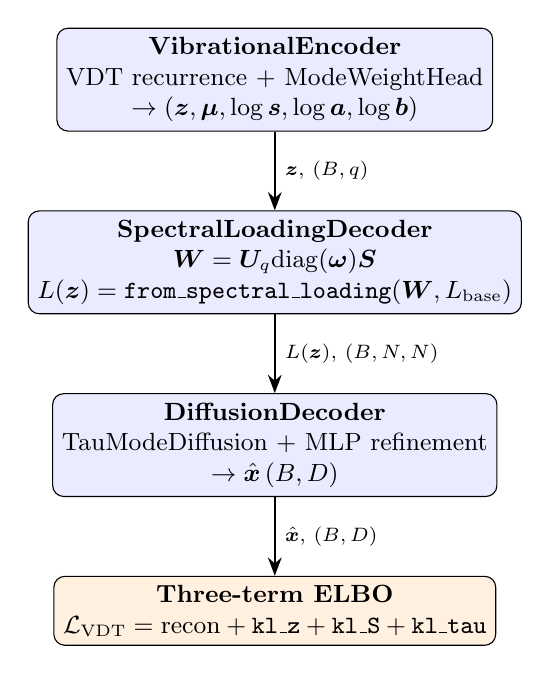
\begin{tikzpicture}[
  box/.style={draw, rounded corners=4pt, fill=blue!8,
              minimum width=5.2cm, minimum height=0.8cm,
              font=\small, align=center},
  sbox/.style={draw, rounded corners=4pt, fill=orange!12,
              minimum width=5.2cm, minimum height=0.8cm,
              font=\small, align=center},
  arr/.style={-Stealth, thick},
]
  \node[box] (enc) {\textbf{VibrationalEncoder}\\VDT recurrence + ModeWeightHead\\$\to (\bz,\bmu,\log\bm{s},\log\bm{a},\log\bm{b})$};
  \node[box, below=1.0cm of enc] (sld) {\textbf{SpectralLoadingDecoder}\\$\bW = \bU_q\diag(\bomega)\bS$\\$L(\bz) = \texttt{from\_spectral\_loading}(\bW, L_{\mathrm{base}})$};
  \node[box, below=1.0cm of sld] (diff) {\textbf{DiffusionDecoder}\\TauModeDiffusion + MLP refinement\\$\to \hat{\bx}\,(B,D)$};
  \node[sbox, below=1.0cm of diff] (loss) {\textbf{Three-term ELBO}\\$\mathcal{L}_{\mathrm{VDT}} = \text{recon} + \texttt{kl\_z} + \texttt{kl\_S} + \texttt{kl\_tau}$};
  \draw[arr] (enc) -- (sld) node[midway,right,font=\scriptsize]{$\bz,\,(B,q)$};
  \draw[arr] (sld) -- (diff) node[midway,right,font=\scriptsize]{$L(\bz),\,(B,N,N)$};
  \draw[arr] (diff) -- (loss) node[midway,right,font=\scriptsize]{$\hat{\bx},\,(B,D)$};
\end{tikzpicture}
\caption{VDT data flow.  The eigenpairs $(\bU_q, \bLambda_q)$ of $L(\I)$
are frozen constants passed to both encoder and decoder; no Laplacian is
computed at runtime.}
\label{fig:dataflow}
\end{figure}

\subsection{VibrationalEncoder}
\label{sec:encoder}

\texttt{VibrationalEncoder} (\texttt{vdt/encoder.py}) replaces the \WA{} MLP
encoder with a VDT (Vibrational Discrete Transformer) recurrence stack:
\begin{enumerate}
  \item \textbf{Input projection}: linear layer mapping $(B,D)\to(B,N{\cdot}d)$,
        reshaped to $(B,N,d)$.
  \item \textbf{VibrationalStateBlocks}: $K$ recurrence layers operating on
        $(B,N,d)$ state matrices using the feature-space Laplacian $L_f$.  The
        recurrence implements a discrete damped wave equation in the graph
        spectral domain: the state evolves as
        $\mathbf{h}_{t+1} = (2\bm{I} - \alpha L_f)\mathbf{h}_t - \mathbf{h}_{t-1}$,
        where $\alpha$ is a learnable damping coefficient.  This is a
        finite-difference discretisation of the wave equation
        $\ddot{\mathbf{u}} + \alpha L_f\mathbf{u} = 0$.
  \item \textbf{Modal projection}: mean-pool output over the node dimension
        after projecting through eigenvectors $\bm{v}\in\R^d$.
  \item \textbf{Readout heads}: separate linear layers producing
        $\bmu,\log\bm{s}$ (for $q(\bz)$) and \texttt{ModeWeightHead}
        producing $(\log\bm{a},\log\bm{b})$ for $q(\bomega)$.
\end{enumerate}
The optional $\lambda$-fingerprint (ArrowSpace spectral histogram of $L(\I)$)
can be concatenated to $\bx$ before the input projection
(\texttt{use\_lambda\_features=True}).

\paragraph{ModeWeightHead.}
A single linear layer \texttt{Linear(feat\_dim, 2q)} splits into
$(\log\bm{a}, \log\bm{b})\in\R^q\times\R^q$.  The Gamma parameters are
obtained as $a_k = e^{\log a_k}>0$, $b_k = e^{\log b_k}>0$.
The mode-weight KL \eqref{eq:kl_tau} is computed from these in
\texttt{vdt/spectral.py:tau\_mode\_kl}.

\paragraph{Signed density matrix.}
During the VDT recurrence each block maintains a signed density matrix
$\varrho_t = \varrho_t^+ - \varrho_t^-$, decomposing the state into
constructive and destructive vibrational contributions (positive and negative
amplitudes).  This object is the discrete analogue of the quantum density
matrix when amplitudes are real-valued rather than complex.  It is used as a
stability diagnostic and, optionally, as the seed for the spectral artefact in
reasoning-focused deployments (Option~6, Section~\ref{sec:tracks}).

\subsection{SpectralLoadingDecoder}
\label{sec:decoder}

\texttt{SpectralLoadingDecoder} (\texttt{vdt/wiring\_decoder.py}) is the
default VDT wiring decoder.  The forward pass computes:
\begin{align}
  \bS &= \texttt{S\_net}(\bz).\text{view}(B,q,q), \label{eq:S_net}\\
  \bomega &= \exp(\texttt{omega\_net}(\bz)), \label{eq:omega_net}\\
  \bW &= \bU_q.\text{unsqueeze}(0)
        \;\texttt{@}\;(\bomega.\text{unsqueeze}(-1)\ast\bS),
        \label{eq:W}\\
  L(\bz) &= \texttt{DifferentiableLaplacian.from\_spectral\_loading}(\bW, L_{\mathrm{base}}).
           \label{eq:Lz}
\end{align}

The \texttt{from\_spectral\_loading} call in \eqref{eq:Lz} constructs the
\emph{combinatorial} Laplacian of the gated normalised adjacency in four
steps:
\begin{align}
  A_{\mathrm{base}} &= (\bm{I} - L_{\mathrm{base}})_+,
    & &\text{recover normalised affinity; clamp negatives to zero,}
    \label{eq:Abase}\\
  g_{ij}(\bz) &= \sigma\!\left(-\|\bW_i - \bW_j\|^2\right),
    & &\text{per-edge gate (sigmoid); } \bW_i\text{ is the }i\text{-th row of }\